\begin{figure}
\begin{center}
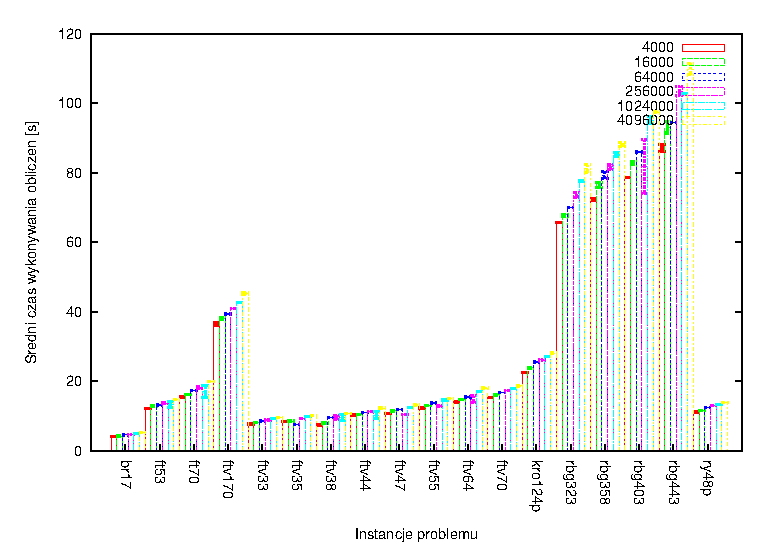
\includegraphics[width=0.9\textwidth]{wykresy/anealing1}
\end{center}
\caption{Średni czas wykonywania obliczeń algorytmu $Simulated Annealing$
dla różnych temperatur początkowych.}
\label{annealing1}
\end{figure}

\begin{figure}
\begin{center}
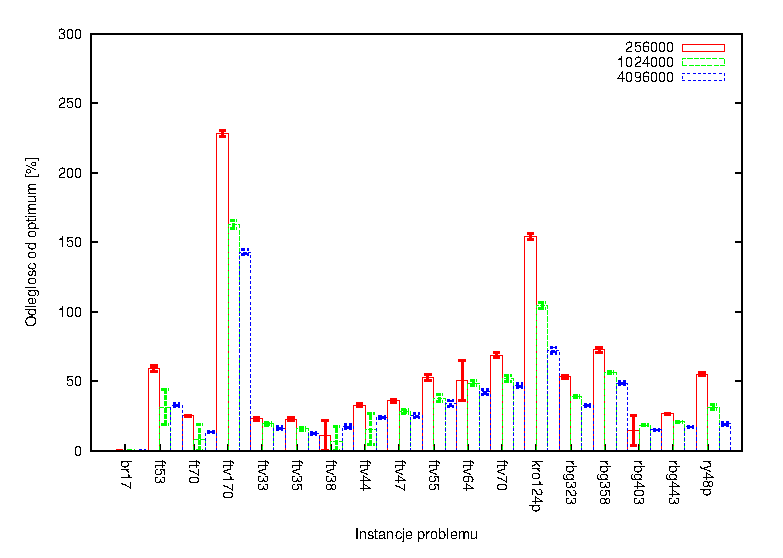
\includegraphics[width=0.9\textwidth]{wykresy/anealing2}
\end{center}
\caption{Odległość od optimum algorytmu $Simulated Annealing$ dla wybranych 
temperatur początkowych.}
\label{annealing2}
\end{figure}

\begin{figure}
\begin{center}
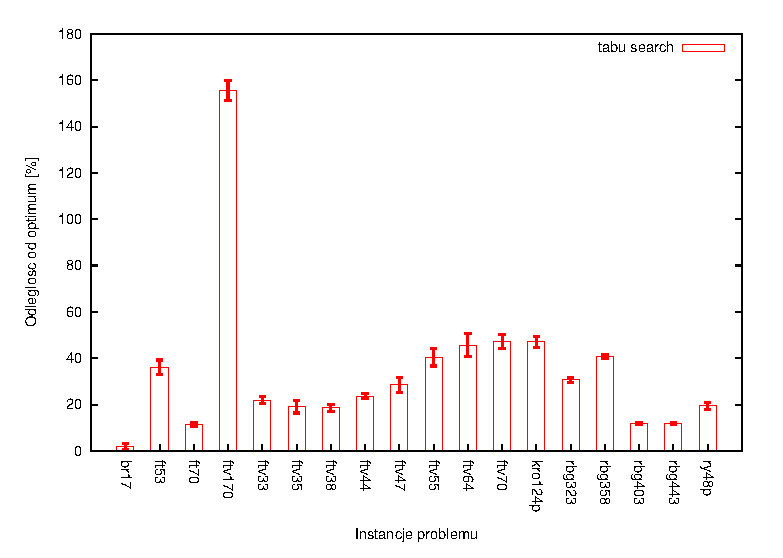
\includegraphics[width=0.9\textwidth]{wykresy/tabu_quality}
\end{center}
\caption{Odległość od optimum algorytmu $Tabu Search$.}
\label{tabu_quality}
\end{figure}

\begin{figure}
\begin{center}
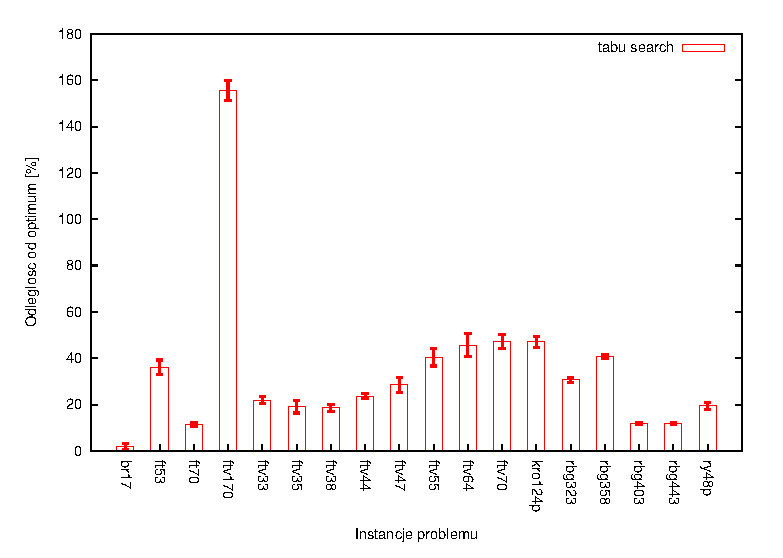
\includegraphics[width=0.9\textwidth]{wykresy/tabu_quality}
\end{center}
\caption{Odległość od optimum algorytmu $Tabu Search$.}
\label{tabu_timeaaaaa}
\end{figure}

\begin{figure}
\begin{center}
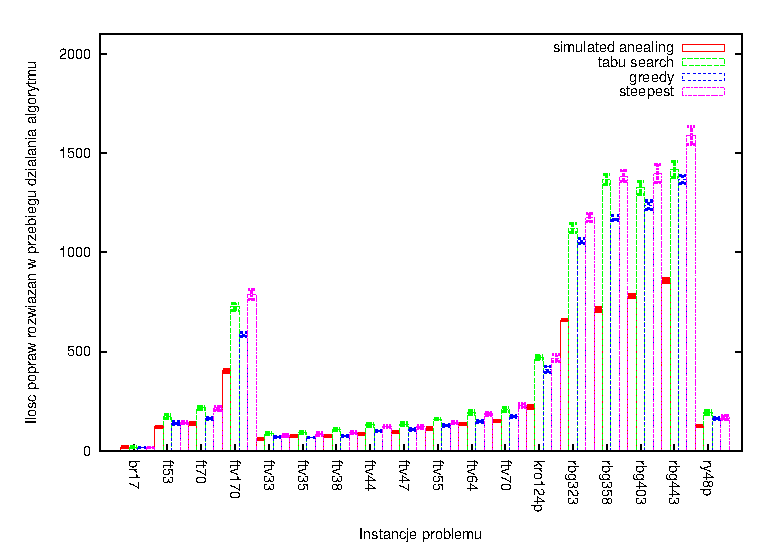
\includegraphics[width=0.9\textwidth]{wykresy/anealing_tabu_greedy_better}
\end{center}
\caption{Ilość popraw rozwiązań w przebiegu działania algorytmów 
$Simulated Annealing$, $Tabu Search$, $Greedy$ i $Steepest$.}
\label{anealing_tabu_greedy_better}
\end{figure}

\begin{figure}
\begin{center}
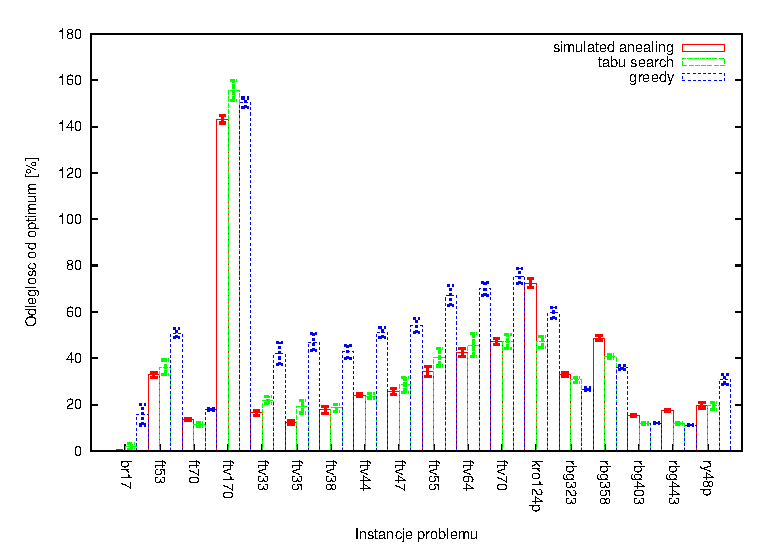
\includegraphics[width=0.9\textwidth]{wykresy/anealing_tabu_greedy_quality}
\end{center}
\caption{Odległość od optimum algorytmów: 
$Simulated Annealing$, $Tabu Search$ i $Greedy$.}
\label{anealing_tabu_greedy_quality}
\end{figure}

\begin{figure}
\begin{center}
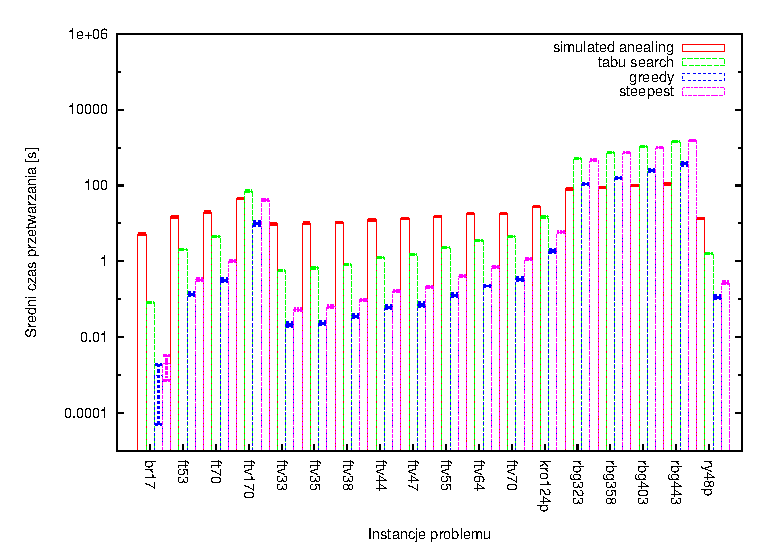
\includegraphics[width=0.9\textwidth]{wykresy/anealing_tabu_greedy_time_log}
\end{center}
\caption{Średni czas przetwarzania algorytmów: 
$Simulated Annealing$, $Tabu Search$, $Greedy$ i $Steepest$.}
\label{anealing_tabu_greedy_time_log}
\end{figure}

\begin{figure}
\begin{center}
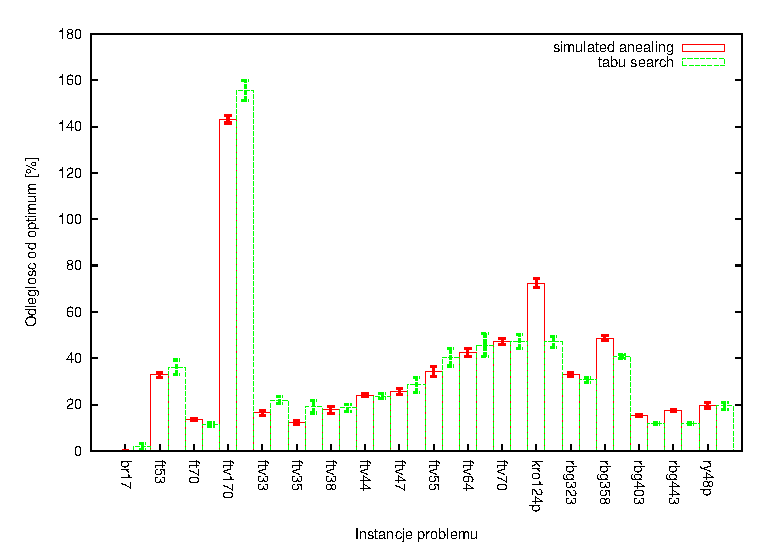
\includegraphics[width=0.9\textwidth]{wykresy/anealing_tabu_quality}
\end{center}
\caption{Odległośc od optimum algorytmów: $Simulated Annealing$ i 
$Tabu Search$.}
\label{anealing_tabu_quality}
\end{figure}

%TS:
\begin{figure}
\begin{center}
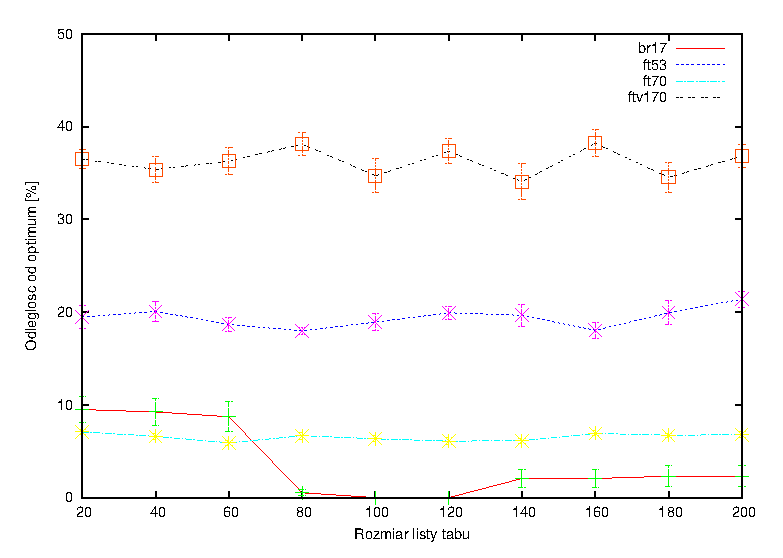
\includegraphics[width=0.9\textwidth]{wykresy/tabu_quality_size_1}
\end{center}
\caption{Odległość od optimum algorytmu $Tabu Search$ dla różnych rozmiarów
listy tabu dla wybranych instancji.}
\label{tabu_quality_size_1}
\end{figure}

\begin{figure}
\begin{center}
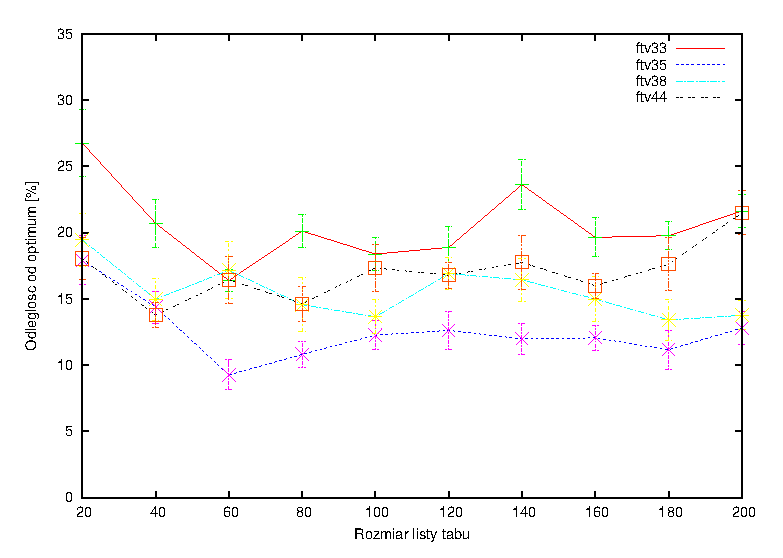
\includegraphics[width=0.9\textwidth]{wykresy/tabu_quality_size_2}
\end{center}
\caption{Odległość od optimum algorytmu $Tabu Search$ dla różnych rozmiarów
listy tabu dla wybranych instancji.}
\label{tabu_quality_size_2}
\end{figure}

\begin{figure}
\begin{center}
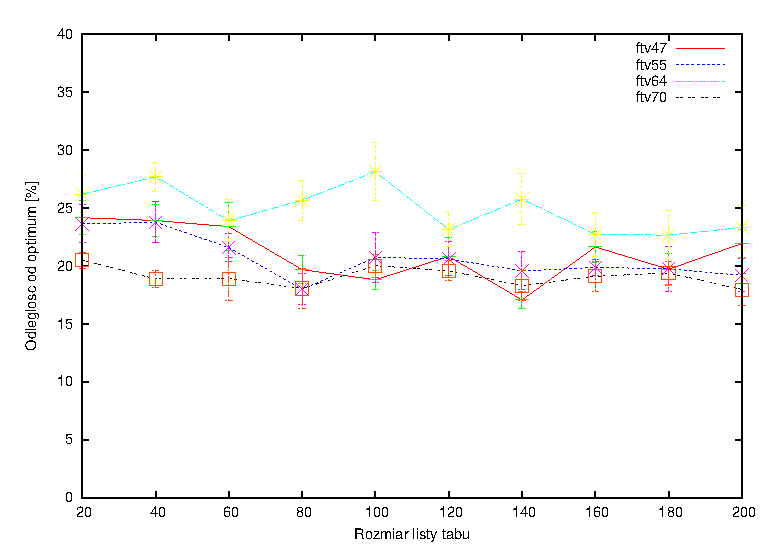
\includegraphics[width=0.9\textwidth]{wykresy/tabu_quality_size_3}
\end{center}
\caption{Odległość od optimum algorytmu $Tabu Search$ dla różnych rozmiarów
listy tabu dla wybranych instancji.}
\label{tabu_quality_size_3}
\end{figure}

\begin{figure}
\begin{center}
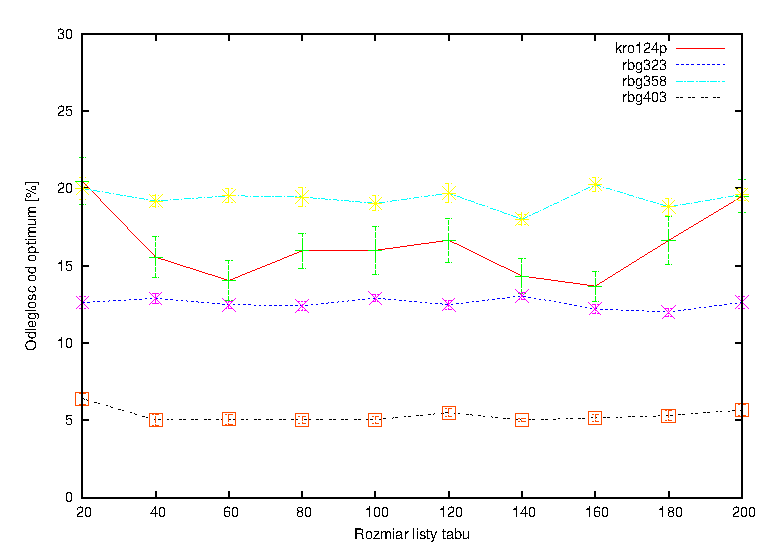
\includegraphics[width=0.9\textwidth]{wykresy/tabu_quality_size_4}
\end{center}
\caption{Odległość od optimum algorytmu $Tabu Search$ dla różnych rozmiarów
listy tabu dla wybranych instancji.}
\label{tabu_quality_size_5}
\end{figure}


\begin{figure}
\begin{center}
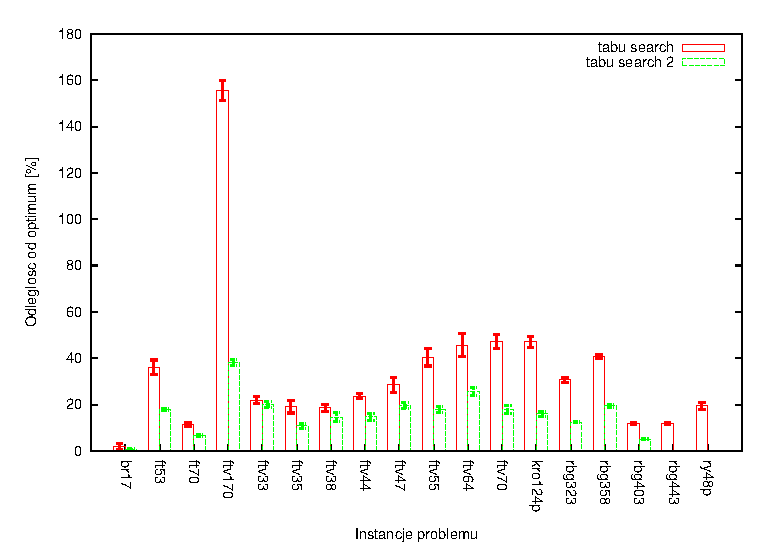
\includegraphics[width=0.9\textwidth]{wykresy/tabu_quality_2}
\end{center}
\caption{Porównanie rozwiązań algorytmu $Tabu Search$ dla różnych rozwiązań
startowych. Wykres opisany jako Tabu Search jest to wykres rozpoczynający
działanie od losowego rozwiązania początkowego. Wykres Tabu Search 2 przedstawia
wyniki działania algorytmu, którego rozwiązaniem początkowym jest wynik 
działania własnego zaproponowanego rozwiązania.}
\label{tabu_quality_2}
\end{figure}